\documentclass[12pt,a4paper]{article}

\usepackage[a4paper,top=2.5cm,bottom=2.5cm,left=2.8cm,right=2.8cm]{geometry}
\usepackage{fontspec}
\usepackage{graphicx,float,booktabs,tabularx,array,longtable}
\usepackage{tikz}
\usetikzlibrary{arrows.meta,positioning,shapes.geometric}
\usepackage{xcolor,listings,enumitem,amsmath,url,hyperref}

\setmainfont{TeX Gyre Termes}
\setsansfont{TeX Gyre Heros}
\setmonofont{DejaVu Sans Mono}
\graphicspath{{figures/}}
\setlength{\parindent}{2em}
\setlength{\parskip}{0.25em}
\linespread{1.22}
\setlength{\emergencystretch}{2em}
\renewcommand{\arraystretch}{1.2}
\setlist{nosep,leftmargin=2em}
\hypersetup{hidelinks}
\newcolumntype{Y}{>{\raggedright\arraybackslash}X}
\definecolor{codegray}{gray}{0.95}
\lstset{basicstyle=\ttfamily\small,backgroundcolor=\color{codegray},frame=single,breaklines=true,columns=fullflexible,keepspaces=true,showstringspaces=false}

\title{\textbf{Experiment 3: Automatic Classification and Arrangement of Desktop Objects}}
\author{Haoran Xiao\\Student ID: 24020036066}
\date{September 12, 2026}

\begin{document}
\maketitle
\thispagestyle{empty}
\begin{center}
Robotic Systems Integration Laboratory\\
Elephant Robotics mechArm 270 Pi, Isaac Sim, ROS 2 Humble, and YOLO
\end{center}
\vfill
\begin{abstract}
This individual report presents the simulation part of Experiment 3, which implements automatic classification and arrangement of tennis balls and green wooden pencils on a circular desktop. The simulated mechArm 270 Pi is placed at the circle centre, while six objects and two open-top bins are arranged on the same ring. A virtual camera observes the scene from above. YOLO is used only to determine the category at a known grid coordinate; the pickup position is never calculated from a YOLO bounding-box centre. The final workflow first buffers six consecutive camera frames and applies a 4-out-of-6 majority vote to all six fixed regions. The locked classes are then used by a ROS 2 sorting state machine to execute the G1--G6 pick-and-place sequence.

The implementation uses Isaac Sim 5.1.0 on Windows, ROS 2 Humble in Docker, and a TCP bridge for joint commands and camera frames. A 13-view camera sweep tested 65 frames using the Experiment 1 YOLO model. The selected 10-degree north-tilted view achieved 6/6 correct fixed-ROI classifications in every tested frame, with mean confidence 0.836. The complete static test suite passed 78 tests after the final G6 scene correction. The main engineering lessons were that fixed-coordinate perception must reproduce the production ROI pipeline, and that generated scene state, YAML configuration, and camera ROIs must be kept synchronized.
\end{abstract}

\noindent\textbf{Keywords:} robotic manipulation; Isaac Sim; ROS 2; fixed-point grasping; YOLO; numerical inverse kinematics

\clearpage
\tableofcontents
\clearpage

\section{Basic Requirements of the Experiment}

The objective of Experiment 3 is to build a simulation in which a robotic arm identifies desktop objects by category and places them into corresponding containers. The required categories in this implementation are \texttt{tennis\_ball} and \texttt{pencil}. The object coordinates are fixed and known in advance. Therefore, visual recognition is responsible only for the semantic category, while the manipulation controller uses pre-calibrated world coordinates.

The final scene contains a square desktop, a mechArm 270 Pi with an adaptive gripper at the centre, six objects on a circular ring, and two open-top bins. Four positions contain tennis balls and two positions contain green wooden pencils. G6 was changed from a pencil to a tennis ball after the first batch test showed that the pencil at that position could not reach the required confidence consistently. This correction preserved the two-category task while improving the robustness of the complete arrangement.

\begin{table}[H]
\centering
\caption{Basic requirements and completion evidence}
\begin{tabularx}{\textwidth}{p{4.0cm}Y p{2.2cm}}
\toprule
Requirement & Implementation and evidence & Status\\
\midrule
Simulated robotic arm and gripper & MechArm 270 Pi and adaptive gripper imported into Isaac Sim; ROS 2 trajectory controller connected through TCP. & Completed\\
Six objects and two bins & Four tennis balls and two pencils are arranged around the robot; the bins are open-top, deep, and physically collidable. & Completed\\
Circular layout & Object and bin centres use fixed coordinates around the robot-centred ring. & Completed\\
Virtual overhead camera & The final camera is 10 degrees tilted toward north, 1.10 m high, and aimed at the ring centre. & Completed\\
Category recognition & YOLO uses fixed image ROIs and six-frame majority voting; it does not calculate pickup coordinates. & Completed\\
Automatic sorting & The controller uses the locked categories to select the tennis or pencil bin and executes G1--G6 in order. & Completed\\
Error handling and records & Unknown classes stop the task safely; camera sweep reports, detections, parameters, and run recordings are retained. & Completed\\
\bottomrule
\end{tabularx}
\end{table}

\section{My Individual Division of Work}

My individual work covered the complete simulation integration rather than only one isolated software module. I first separated Experiment 3 into its own workspace so that the Experiment 2 files and environment remained untouched. I then adapted the existing mechArm model and built the circular experiment scene, including the desktop, the object ring, the two deep bins, the pencil geometry, object collision bodies, and friction materials.

I was responsible for the following work:

\begin{enumerate}
  \item \textbf{Scene and physical modelling:} created the centred ring layout, open bins with collision walls, tennis balls, and a composite green wooden pencil with a cylindrical shaft, wood tip, and graphite tip. I added collision geometry for the pencil and tuned the object--gripper friction.
  \item \textbf{Camera and perception:} connected the Isaac camera stream to ROS 2, reused the Experiment 1 YOLO model, synchronised fixed image ROIs with the tilted camera, and designed the six-frame majority-vote calibration process.
  \item \textbf{Manipulation control:} retained the Experiment 2 mechArm parameters, numerical IK, smooth quintic interpolation, separate fast and slow motion speeds, lift clearance, direct release above the bin, and final HOME return.
  \item \textbf{ROS 2 and Docker integration:} implemented the launch flow, TCP joint bridge, trajectory controller, virtual camera node, YOLO node, sorting state machine, recorder, and Docker build environment.
  \item \textbf{Testing and evidence:} wrote contract and unit tests, performed the 13-view camera sweep, recorded detection metrics, preserved representative scene frames, and maintained the local GitHub repository for Experiment 3.
\end{enumerate}

\section{Principles of the Project Implementation}

\subsection{System Architecture}

The system is divided into a Windows Isaac Sim process and a Dockerised ROS 2 process. Isaac Sim owns the scene, rigid-body dynamics, robot articulation, camera rendering, and TCP server. ROS 2 owns the visual classification, fixed-coordinate target generation, trajectory interpolation, task sequencing, and result recording.

\begin{figure}[H]
\centering
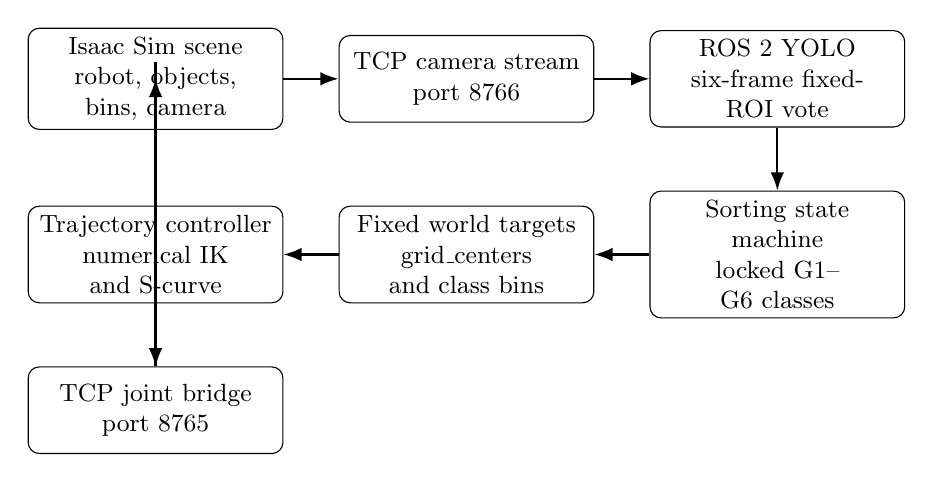
\begin{tikzpicture}[
  node distance=8mm and 7mm,
  box/.style={draw,rounded corners,minimum height=11mm,text width=3.0cm,align=center,font=\small},
  arrow/.style={-Latex,thick}
]
\node[box] (scene) {Isaac Sim scene\\robot, objects, bins, camera};
\node[box,right=of scene] (camera) {TCP camera stream\\port 8766};
\node[box,right=of camera] (vision) {ROS 2 YOLO\\six-frame fixed-ROI vote};
\node[box,below=of vision] (state) {Sorting state machine\\locked G1--G6 classes};
\node[box,left=of state] (target) {Fixed world targets\\grid\_centers and class bins};
\node[box,left=of target] (motion) {Trajectory controller\\numerical IK and S-curve};
\node[box,below=of motion] (bridge) {TCP joint bridge\\port 8765};
\draw[arrow] (scene) -- (camera);
\draw[arrow] (camera) -- (vision);
\draw[arrow] (vision) -- (state);
\draw[arrow] (state) -- (target);
\draw[arrow] (target) -- (motion);
\draw[arrow] (motion) -- (bridge);
\draw[arrow] (bridge) |- (scene);
\end{tikzpicture}
\caption{Data and control flow of the Experiment 3 simulation}
\label{fig:architecture}
\end{figure}

\subsection{Circular Layout and Fixed Coordinates}

The robot is located at the origin of the desktop coordinate system. The six object centres and two bin centres are specified in \texttt{config/experiment3\_sorting.yaml}. The controller uses these values directly. For a grid $G_i$, the pickup command is
\begin{equation}
  \mathbf{p}_i = [x_i,y_i,z_i]^T = \texttt{grid\_centers}[G_i].
\end{equation}
The class returned by YOLO selects the bin, but neither the YOLO image coordinate nor the detected box size changes $\mathbf{p}_i$.

\begin{figure}[H]
\centering
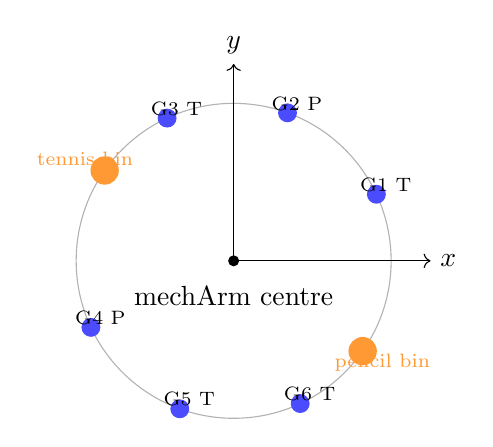
\begin{tikzpicture}[scale=2.0]
  \draw[gray!60] (0,0) circle (1.0);
  \fill[black] (0,0) circle (0.035) node[below=2mm] {mechArm centre};
  \foreach \a/\id/\type in {25/G1/T,70/G2/P,115/G3/T,205/G4/P,250/G5/T,295/G6/T}{
    \coordinate (c\id) at (\a:1.0);
    \fill[blue!70] (c\id) circle (0.06);
    \node[font=\scriptsize] at (c\id) [shift={(0.12,0.12)}] {\id~\type};
  }
  \fill[orange!80] (145:1.0) circle (0.09) node[font=\scriptsize,shift={(-0.25,0.15)}] {tennis bin};
  \fill[orange!80] (325:1.0) circle (0.09) node[font=\scriptsize,shift={(0.25,-0.15)}] {pencil bin};
  \draw[->] (0,0) -- (0:1.25) node[right] {$x$};
  \draw[->] (0,0) -- (90:1.25) node[above] {$y$};
\end{tikzpicture}
\caption{Schematic of the robot-centred circular arrangement; T denotes tennis ball and P denotes pencil.}
\label{fig:ring}
\end{figure}

\subsection{Camera and Fixed-ROI YOLO Recognition}

The production camera uses a resolution of $848\times480$, focal length 18 mm, and height 1.10 m. A sweep tested 13 candidates: vertical, then 10, 15, and 20 degree tilts from four azimuth directions. Each candidate produced five frames. The winning camera is positioned at approximately $(0,0.19396,1.10)$ m and looks at the origin.

The recognition pipeline is intentionally different from visual servoing. The six object locations are known. For each frame, the classifier crops the configured ROI for the requested grid and runs YOLO on that crop. After six frames, the node counts class votes. A class is accepted only if it is the unique winner with at least four votes. The sorting node receives six semantic decisions in one message, stores them, and then uses the fixed grid order for motion.

\begin{figure}[H]
\centering
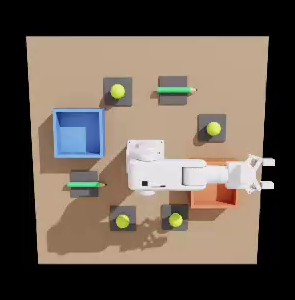
\includegraphics[width=.72\textwidth,keepaspectratio]{final_scene_initial.png}
\caption{Final Experiment 3 scene after replacing G6 with a tennis ball. The robot is at the centre and the six objects and two bins surround it.}
\label{fig:scene}
\end{figure}

\subsection{Manipulation and Motion Planning}

The motion controller follows the stable strategy used in Experiment 2. The target pose is solved numerically while preserving the tool-axis constraint. Ordinary horizontal motion uses 20 deg/s and the final vertical approach, closure, lift, and release-related movement use 3 deg/s. A quintic smoothstep profile reduces acceleration discontinuities:
\begin{equation}
  s(t)=10\tau^3-15\tau^4+6\tau^5, \qquad \tau=t/T,\quad 0\leq\tau\leq1.
\end{equation}
For each object the arm moves to a pre-grasp height, descends slowly to the fixed grasp height, closes the gripper, lifts to $z=0.133$ m, moves above the selected bin, opens the gripper to release the object, and proceeds directly to the next grid. The robot returns HOME only after G6.

\section{Problems Encountered and Solutions}

\subsection{Camera Sweep Initially Produced Black Frames}

The first sweep created 65 image files, but pixel inspection showed that all images had maximum intensity 0. Treating those files as valid evidence would have produced a false YOLO conclusion. The cause was that the sweep used an independent Replicator camera and advanced Replicator steps without following the normal Isaac \texttt{World.step(render=True)} loop. I changed the sweep to reuse the existing scene camera, initialise an Isaac \texttt{World}, play the world, and wait for rendered frames. I also added a non-black frame validator that aborts instead of recording invalid evidence. The second sweep produced 65 non-black images.

\subsection{Full-Image YOLO Was the Wrong Evaluation Boundary}

When the model was run on the complete $848\times480$ image, it detected tennis balls but returned no pencils. This initially suggested that camera angle alone could not solve the problem. I compared the classifier implementation and found that the production node already cropped a fixed ROI before YOLO inference. Re-evaluating each known grid ROI reproduced the actual runtime boundary and recovered pencil detections. This changed the sweep evaluator from full-image detection counting to projected fixed-ROI classification. The result was more meaningful and directly connected to the real sorting pipeline.

\subsection{The 90-Degree View Was Not Uniformly Robust}

The original vertical view was visually clear, but two pencil positions had weak confidence. I tested 13 views with the same model and threshold. The 10-degree north view achieved 6/6 correct decisions in all five frames and raised the weak pencil confidences. The camera pose and all world pickup coordinates were then synchronised with the selected view. This was a useful example of separating geometric calibration from learned detection: the camera changed, but the robot did not chase image coordinates.

\subsection{Batch Recognition Revealed an Unstable G6 Pencil}

After changing the controller to classify all six grids before motion, the first runtime batch produced stable results for G1--G5 but marked G6 unknown: its six votes did not reach the required four-vote threshold. I intentionally kept the safety stop instead of forcing a class or grabbing blindly. Since the experiment only requires the two categories and G6 is a fixed design position, I replaced the unstable G6 pencil with a tennis ball, regenerated the USD scene, and updated the YAML object record, ROI shape, and colour metadata. A later runtime capture then showed G6 classified as a tennis ball with 6/6 votes.

\subsection{Middleware, Packaging, and Numerical Issues}

Several lower-level issues also required engineering decisions:
\begin{itemize}
  \item A Docker build failed because a ROS package download returned HTTP 502. Retrying the package installation resolved the transient registry failure.
  \item The Python environment initially contained NumPy 2.x while the ROS cv\_bridge binary had been compiled against NumPy 1.x. Downgrading to NumPy 1.21.5 removed the binary API warning and restored cv\_bridge compatibility.
  \item PowerShell quoting caused false syntax errors when Python code contained nested quotes. I changed the verification commands to use the container's direct Python entry point and simpler quoting.
  \item Isaac reported unresolved visual references and PhysX iteration warnings. They did not stop the TCP state stream; I recorded them as non-blocking warnings and kept the robot and camera data paths under observation.
  \item One early execution stopped at numerical IK because the requested pose was near the orientation boundary. The final controller preserves the Experiment 2 arm parameters and uses safe pre-grasp/lift heights rather than relaxing the physical constraints blindly.
\end{itemize}

These problems shaped my implementation choices. I used evidence gates for images, fixed coordinate contracts for grasping, explicit safe-stop behaviour for uncertain perception, and repeated static tests after each structural change. This made the system easier to explain and reduced the risk of a visually plausible but physically incorrect result.

\section{Verification and Results}

\subsection{Camera View Sweep}

The final sweep used the Experiment 1 model \texttt{pencil\_tennis\_yolo26n\_best.pt}, confidence threshold 0.05, six fixed ROIs, and 65 valid frames. The selected 10-degree north view achieved the following verified result:

\begin{table}[H]
\centering
\caption{Camera sweep result}
\begin{tabular}{ll}
\toprule
Metric & Result\\
\midrule
Candidate views & 13\\
Frames per view & 5\\
Total valid frames & 65\\
Best view & 10-degree north tilt\\
Minimum correct objects per frame & 6/6\\
Pencil recall & 1.000\\
Tennis-ball recall & 1.000\\
Mean confidence & 0.836\\
\bottomrule
\end{tabular}
\end{table}

The report directory contains the full ranking CSV, per-grid detections, camera recommendation YAML, model checksum, application record, and representative annotated frames. The camera sweep evidence is therefore reproducible rather than based on a single favourable image.

\subsection{Batch Recognition and Runtime Evidence}

The first batch runtime after implementation produced G1 tennis ball, G2 pencil, G3 tennis ball, G4 pencil, G5 tennis ball, and G6 unknown. The resulting safe stop demonstrated that the 4/6 rule was active. After replacing G6 with a tennis ball, a subsequent recorded run showed G1--G6 all classified with 6/6 votes, including G6 as \texttt{tennis\_ball}. The run recorder's summary CSV was empty because the capture ended during execution, so I do not claim a completed six-cycle success count from that file. The video and terminal evidence do verify the batch request, six grid classifications, and the beginning of the fixed-coordinate pick sequence.

\begin{figure}[H]
\centering
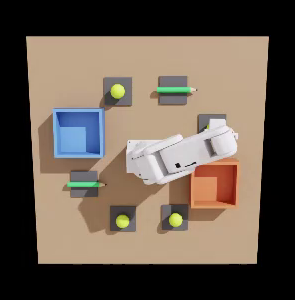
\includegraphics[width=.72\textwidth,keepaspectratio]{final_scene_motion.png}
\caption{Representative runtime frame while the robot executes the fixed-coordinate manipulation sequence.}
\label{fig:motion}
\end{figure}

\subsection{Software Verification}

The final local test command ran both the Experiment 3 tests and the ROS package tests:
\begin{lstlisting}[caption={Final static verification command}]
$env:PYTHONPATH='<experiment3-root>/src/mecharm_pick_place'
python -m pytest <experiment3-root>/tests <experiment3-root>/src/mecharm_pick_place/test -q
\end{lstlisting}
It returned 78 passed tests. Python compilation also passed for the modified Isaac and ROS 2 modules, and the Docker colcon build completed for both \texttt{mecharm\_pick\_place} and \texttt{mycobot\_description}.

\section{Conclusion}

I completed an independent Experiment 3 simulation package for automatic circular arrangement sorting with a mechArm 270 Pi. The final implementation combines a robot-centred ring scene, open deep bins, tennis-ball and green-pencil models, a calibrated tilted virtual camera, fixed-ROI YOLO classification, six-frame majority voting, fixed-world-coordinate manipulation, numerical IK, smooth motion, safe-stop handling, and final HOME return.

The most important design decision was to keep perception and manipulation responsibilities separate. YOLO answers ``what category is at this known grid?''; it does not answer ``where should the robot grasp?''. This makes the system more stable, easier to test, and consistent with the fixed-coordinate experimental requirement. The 13-view sweep achieved 6/6 classification in every tested frame for the selected view, and 78 static tests passed after the final scene correction.

The remaining limitation is that the recorded runtime summary did not contain a complete per-object success table, so a future acceptance run should preserve one machine-readable result for each of the six placements. A further improvement would be to attach the per-frame vote history directly to the recorder output and add a single command that starts Isaac, ROS 2, and the batch sorting task with explicit readiness checks.

\section*{References}
\addcontentsline{toc}{section}{References}
\begingroup\sloppy
\begin{enumerate}
  \item NVIDIA, ``Isaac Sim Documentation, Version 5.1.0,'' \url{https://docs.isaacsim.omniverse.nvidia.com/5.1.0/}.
  \item Open Robotics, ``ROS 2 Humble Documentation,'' \url{https://docs.ros.org/en/humble/}.
  \item Elephant Robotics, ``myCobot ROS 2 Package,'' \url{https://github.com/elephantrobotics/mycobot_ros2}.
  \item Ultralytics, ``Ultralytics YOLO Documentation,'' \url{https://docs.ultralytics.com/}.
  \item Experiment 3 local repository, ``mecharm-experiment3-sorting,'' \url{https://github.com/xhr-CHN/mecharm-experiment3-sorting}.
\end{enumerate}
\endgroup

\end{document}
